% ============================================================
% GSPH-FC (v2) — Springer LNCS — VERSIÓN EN ESPAÑOL
% Traducción de samplepaper_v2.tex (mismos datos, tablas y figuras).
% Compilar: pdflatex -> bibtex -> pdflatex -> pdflatex
% Figuras en Resultados_v2/ (generadas con experiments/algorithms/GSPH_V2.py)
% Números de las tablas: experiments/results/v2/benchmark_v2.csv y
% experiments/results/{ablacion,sensibilidad,lkh}/
% ============================================================
\documentclass[runningheads]{llncs}
\usepackage[T1]{fontenc}
\usepackage[utf8]{inputenc}
\usepackage[spanish,es-tabla,es-noshorthands,es-nodecimaldot]{babel}
\usepackage{graphicx}
\usepackage{amsmath,amssymb}
\usepackage{booktabs}
\usepackage{algorithm}
\usepackage[noend]{algpseudocode}
\usepackage{url}

\floatname{algorithm}{Algoritmo}
\algrenewcommand\algorithmicrequire{\textbf{Entrada:}}
\algrenewcommand\algorithmicensure{\textbf{Salida:}}
\algrenewcommand\algorithmicwhile{\textbf{mientras}}
\algrenewcommand\algorithmicdo{\textbf{hacer}}
\algrenewcommand\algorithmicforall{\textbf{para todo}}
\algrenewcommand\algorithmicif{\textbf{si}}
\algrenewcommand\algorithmicthen{\textbf{entonces}}
\algrenewcommand\algorithmicelse{\textbf{si no}}
\algrenewcommand\algorithmicreturn{\textbf{devolver}}
\AtBeginDocument{\renewcommand\keywordname{{\bfseries Palabras clave:}}}

\begin{document}

\title{GSPH-FC: una heurística de partición geométrica del espacio
con conectividad de fronteras para el TSP euclidiano}
\titlerunning{GSPH-FC: partición geométrica del espacio para el TSP}

\author{%
    Martín Gómez Navarro\inst{1} \and
    Rodrigo Linfati\inst{2} \and
    Juan Carlos Figueroa-García\inst{3} \and
    Carlos Alberto Franco Franco\inst{3} \and
    Daniel Morillo-Torres\inst{4} \and
    Jairo R. Coronado-Hernandez\inst{5} \and
    Gustavo Esteban Gatica\inst{1}}
\authorrunning{M. Gómez Navarro et al.}
\institute{%
    Facultad de Ingeniería, Universidad Andrés Bello, Santiago, Chile\\
    \email{m.gmeznavarro@uandresbello.edu}\\
    \email{ggatica@uandresbello.edu}
    \and
    Facultad de Ingeniería, Universidad del Bío-Bío,
    Concepción, Chile\\
    \email{rlinfati@ubiobio.cl}
    \and
    Facultad de Ingeniería, Universidad Distrital
    Francisco José de Caldas, Bogotá, Colombia\\
    \email{jcfigueroag@udistrital.edu.co}
    \email{cafrancof@udistrital.edu.co}
    \and
    Facultad de Ingeniería, Pontificia Universidad Javeriana de Cali,
    Cali, Colombia\\
    \email{daniel.morillo@javerianacali.edu.co}
    \and
    Facultad de Ingeniería, Universidad de la Costa,
    Barranquilla, Colombia\\
    \email{jcoronad18@cuc.edu.co}}

\maketitle

\begin{abstract}
Proponemos \textbf{GSPH-FC} (\textit{Geometric Space Partitioning with
Frontier Connectivity}), una heurística geométrica para el problema del
vendedor viajero (TSP) euclidiano. El método divide el plano en cuatro
cuadrantes, elige pares de nodos que conectan cuadrantes vecinos (pares
de frontera) y construye dentro de cada cuadrante caminos anclados cuyos
extremos quedan fijados por esas decisiones de frontera. El tour
ensamblado se mejora con una búsqueda local iterada (ILS) que combina
2-opt y Or-opt con listas de vecinos, una perturbación double-bridge
\emph{localizada} cuya ventana crece con el tamaño de la instancia, una
regla de aceptación tipo Metropolis y un criterio de parada por
estancamiento. Todos los núcleos de búsqueda trabajan sobre arreglos de
índices y se compilan a código nativo, y las perturbaciones rechazadas se
deshacen mediante un registro de inversiones de segmentos en vez de
copiar el tour. En 77 instancias de TSPLIB de hasta 18\,512 ciudades con
la métrica \texttt{EUC\_2D}, el método alcanza la mejor solución conocida
(BKS) en 44 instancias y en todas las de $n\le 300$; el mejor tour queda
a menos de 0.60\% de la BKS en todas las instancias de hasta 6\,000
ciudades. Frente a nuestra implementación anterior, en las 37 instancias
que esta reportaba, el GAP promedio del mejor tour baja de 0.080\% a
0.000\% (las 37 en la BKS) y el tiempo por ejecución cae de 14.65~s a
0.23~s, unas 65 veces más rápido. Una ablación que mantiene fijo el motor
de búsqueda muestra que la conectividad de fronteras entrega los mejores
tours iniciales (9.95\% sobre la BKS frente a 24.71\% del vecino más
cercano) y la mayor cantidad de aciertos de la BKS, pero que la mayor
parte de la calidad final se debe al ILS localizado. LKH-3 sigue siendo
más preciso, sobre todo por encima de 300 ciudades.
\keywords{2-opt \and Conectividad de fronteras \and Descomposición
geométrica \and Búsqueda local iterada \and Instancias TSPLIB \and
Problema del vendedor viajero}
\end{abstract}

% ================================================================
\section{Introducción}
% ================================================================

El \textit{problema del vendedor viajero} (TSP) euclidiano busca un
ciclo hamiltoniano de largo mínimo que pase por $n$ puntos del plano, y
sigue siendo uno de los bancos de prueba más clásicos para el diseño de
heurísticas en optimización
combinatoria~\cite{applegate2006tsp,laporte1992tsp}. Aunque los métodos
exactos resuelven a optimalidad muchas instancias de prueba, las
heurísticas siguen siendo relevantes cuando se buscan métodos
interpretables, escalables y livianos, con una estructura de diseño
explícita en vez de mucha maquinaria
oculta~\cite{garey1979computers,mardones2023}.

La hipótesis central de \textbf{GSPH-FC} (\textit{Geometric Space
Partitioning with Frontier Connectivity}) es que la estructura
geométrica debe guiar no solo la \emph{ubicación} de los subproblemas,
sino también el \emph{ensamblaje} de sus soluciones locales. Por eso la
conectividad de fronteras es un principio de construcción de primer
orden: los pares de frontera se eligen antes de construir las rutas
locales y se usan como anclas obligatorias de entrada y salida de los
caminos dentro de cada cuadrante.

Una primera implementación de esta idea ya alcanzaba la BKS en muchas
instancias pequeñas, pero gastaba un presupuesto de tiempo fijo por
ejecución (5--30~s) aunque la búsqueda ya hubiera convergido, realizaba
solo unos cientos de iteraciones de ILS por segundo y se estancaba en
óptimos locales profundos en las instancias medianas. Este trabajo
presenta un método rediseñado que mantiene intacta la construcción
geométrica y reconstruye el motor de mejora en torno a cuatro ideas:
(i) búsqueda local compilada con listas de vecinos y cálculo incremental
del largo, (ii) un double-bridge localizado cuya ventana crece con $n$,
(iii) un criterio de aceptación tipo Metropolis en el espíritu de las
cadenas de Markov de paso
largo~\cite{martin1991large,kirkpatrick1983optimization} y (iv) parada
por estancamiento en vez de por un presupuesto de tiempo.

\paragraph{Contribuciones.}
\begin{enumerate}
  \item \textbf{Ensamblaje anclado guiado por fronteras:} una heurística
    geométrica para el TSP en la que los pares de frontera se eligen
    antes de construir las rutas locales y definen las anclas de entrada
    y salida de cada cuadrante.
  \item \textbf{Un motor de pulido eficiente:} un ILS con parada por
    estancamiento, perturbaciones double-bridge localizadas, aceptación
    de Metropolis y deshacer mediante un registro de inversiones,
    ejecutado por núcleos compilados sobre arreglos de índices.
  \item \textbf{Evidencia empírica amplia:} resultados en 77 instancias
    de TSPLIB de hasta 18\,512 ciudades; una ablación que reemplaza la
    construcción manteniendo fijo el motor de búsqueda, para separar el
    aporte de la conectividad de fronteras del aporte del ILS; un estudio
    de sensibilidad de parámetros, uno a la vez; una comparación con
    LKH-3; y una comparación con la implementación anterior que muestra
    mejoras simultáneas en calidad y velocidad.
\end{enumerate}

El resto del trabajo se organiza así. La Sección~\ref{sec:related}
revisa los antecedentes. La Sección~\ref{sec:formulation} presenta la
formulación geométrica. La Sección~\ref{sec:algorithm} describe el
algoritmo y su implementación. La Sección~\ref{sec:experiments} reporta
los resultados experimentales. La Sección~\ref{sec:analysis} discute
fortalezas y limitaciones, y la Sección~\ref{sec:conclusions} concluye.

% ================================================================
\section{Trabajo relacionado}
\label{sec:related}
% ================================================================

GSPH-FC se basa en ideas de heurísticas geométricas para el TSP,
búsqueda local y metaheurísticas de trayectoria. El vecino más cercano
(NN) es la línea base constructiva clásica: corre en $O(n^2)$ y se usa a
menudo como punto de partida de heurísticas de mejora, pero por sí solo
suele quedar lejos del óptimo~\cite{kizilatecs2013nearest}. La
heurística 2-opt mejora un tour invirtiendo segmentos que acortan el
largo total~\cite{croes1958method}; junto con listas de candidatos y
Don't-Look Bits, sigue siendo uno de los componentes más importantes de
la búsqueda local euclidiana~\cite{johnson1997tsp,bentley1992fast}.
Or-opt reubica segmentos cortos y complementa a 2-opt a bajo
costo~\cite{or1976traveling}. La familia Lin--Kernighan y sus
descendientes, como LKH, extienden estas ideas a vecindarios de
profundidad variable y están entre las heurísticas prácticas más
fuertes para el
TSP~\cite{lin1973effective,helsgaun2000effective,helsgaun2017extension}.

A un nivel más alto, muchas metaheurísticas alternan perturbación y
mejora local para escapar de óptimos locales. La búsqueda local iterada
(ILS) combina una búsqueda local fuerte con una diversificación liviana
mediante perturbaciones~\cite{lourencco2003ils}. En el TSP, los
double-bridge seguidos de reoptimización local son una combinación
particularmente exitosa, y la cadena de Markov de paso largo de Martin,
Otto y Felten acepta soluciones peores con una probabilidad tipo
Boltzmann~\cite{martin1991large}, un mecanismo tomado del recocido
simulado~\cite{kirkpatrick1983optimization}. GSPH-FC sigue esta línea,
pero agrega una capa explícita de descomposición geométrica y hace que
la conectividad de fronteras forme parte de la construcción misma de las
rutas locales.

La descomposición geométrica también tiene una larga historia. El
algoritmo de partición de Karp divide el plano recursivamente en celdas,
resuelve cada celda y une los subtours, con garantías probabilísticas
para puntos uniformes~\cite{karp1977probabilistic}. Las heurísticas de
curvas que llenan el espacio visitan los puntos en el orden de una curva
recursiva por cuadrantes en tiempo
$O(n\log n)$~\cite{bartholdi1982spacefilling}. POPMUSIC descompone un
tour existente en subproblemas superpuestos que se reoptimizan por
separado, y lo usa para construir listas de candidatos para
LKH~\cite{taillard2019popmusic}. En todos estos métodos, las conexiones
entre regiones son un subproducto: salen de la unión de subtours, del
orden de una curva o se heredan de un tour previo. GSPH-FC se diferencia
en que las conexiones entre cuadrantes vecinos se eligen explícitamente,
antes de que existan las rutas locales, y luego se imponen como extremos
fijos de esas rutas. La Sección~\ref{sec:ablation} mide cuánto aporta
esta decisión cuando se aplica un motor de mejora fuerte.

Por lo tanto, no afirmamos que NN, 2-opt, Or-opt o ILS sean novedosos
por separado. La contribución está en la forma en que la partición
geométrica, el anclaje guiado por fronteras y un ILS localizado
eficiente se combinan en un método geométrico coherente.

\begin{table}
\caption{Principales familias de métodos para el TSP y sus
compromisos cualitativos.}
\label{tab:comparison}
\centering\small
\begin{tabular}{@{}lllll@{}}
\toprule
\textbf{Método} & \textbf{Tipo} & \textbf{Complejidad} & \textbf{Escalabilidad} & \textbf{Calidad} \\
\midrule
Fuerza bruta          & Exacto        & $O(n!)$      & Muy baja  & Óptima \\
Programación dinámica & Exacto        & $O(n^2 2^n)$ & Baja      & Óptima \\
Vecino más cercano    & Constructivo  & $O(n^2)$     & Alta      & Baja \\
2-opt                 & Mejora        & $O(n^2)$/iter& Media     & Media \\
Lin--Kernighan/LKH    & Mejora        & Variable     & Alta      & Muy alta \\
Heurísticas tipo ILS  & Metaheurística & Variable    & Alta      & Alta \\
\textbf{GSPH-FC}      & Heurística geométrica & $O(n^2)+O(K\cdot\text{iter})^{*}$ & Alta & Alta \\
\bottomrule
\multicolumn{5}{@{}l}{\scriptsize $^{*}$Construcción más $K$ iteraciones de ILS; ver Sección~\ref{sec:complexity}.}
\end{tabular}
\end{table}

% ================================================================
\section{Formulación matemática}
\label{sec:formulation}
% ================================================================

Sea $G=(V,E)$ un grafo completo no dirigido con
$V=\{v_1,\dots,v_n\}\subset\mathbb{R}^2$ y coordenadas $(x_i,y_i)$.
Los costos de las aristas siguen la convención \texttt{EUC\_2D} de
TSPLIB~\cite{reinelt1991tsplib}:
\begin{equation}
 d(v_i,v_j)=\left\lfloor\sqrt{(x_i-x_j)^2+(y_i-y_j)^2}+0.5\right\rfloor.
 \label{eq:dist}
\end{equation}
El TSP busca un ciclo hamiltoniano
$\pi=(v_{\pi(1)},\dots,v_{\pi(n)},v_{\pi(1)})$ que minimice
\begin{equation}
 \min_{\pi}\;L(\pi)=\sum_{i=1}^{n}
 d\!\left(v_{\pi(i)},v_{\pi(i\bmod n+1)}\right).
 \label{eq:tsp}
\end{equation}

\paragraph{Alcance y supuestos.}
Nos limitamos a instancias euclidianas planas con la convención de
redondeo \texttt{EUC\_2D}. Todos los GAP se calculan contra valores de
BKS en la misma métrica.

\subsection{Descomposición geométrica}

Sea el punto medio de la caja envolvente
\begin{equation}
 x_m=\tfrac{x_{\min}+x_{\max}}{2}, \qquad
 y_m=\tfrac{y_{\min}+y_{\max}}{2}.
\end{equation}
La instancia se divide en cuatro cuadrantes:
\begin{align}
Q_1&=\{v\in V: x_v\le x_m,\; y_v>y_m\}  &&\text{(NO)},\\
Q_2&=\{v\in V: x_v>x_m,\; y_v>y_m\}    &&\text{(NE)},\\
Q_3&=\{v\in V: x_v\le x_m,\; y_v\le y_m\}&&\text{(SO)},\\
Q_4&=\{v\in V: x_v>x_m,\; y_v\le y_m\} &&\text{(SE)}.
\end{align}
El método evalúa un pequeño portafolio de estas particiones (de tres a
cinco, menos para $n$ grande) tomadas del punto medio de la caja, la
mediana por coordenada y cuatro puntos medios desplazados en un 12\% del
lado de la caja hacia cada diagonal. Cada candidata sigue siendo una
descomposición en cuatro partes alineada con los ejes.

\subsection{Conectividad de fronteras}

Para cuadrantes vecinos $Q_a,Q_b$, se define una banda de frontera en
torno al borde común. Para una frontera vertical en $x_m$:
\begin{equation}
F_a(\varepsilon)=\{u\in Q_a:|x_u-x_m|<\varepsilon\}, \qquad
F_b(\varepsilon)=\{v\in Q_b:|x_v-x_m|<\varepsilon\}.
\end{equation}
El mejor par de frontera es entonces
\begin{equation}
(u^*,v^*)=\arg\min_{u\in F_a,\,v\in F_b} d(u,v).
\label{eq:frontier}
\end{equation}
Si una banda de frontera está vacía, $\varepsilon$ se duplica hasta
cuatro veces. El método guarda los tres mejores pares de cada frontera y
los combina entre las cuatro fronteras, ordenando las combinaciones por
el largo total de frontera. Lo crucial es que los pares de frontera se
eligen \emph{antes} de construir las rutas locales, de modo que definen
las anclas reales de los caminos locales.

\subsection{Construcción anclada dentro de cada cuadrante}

Dado un cuadrante $Q_k$ y dos anclas $s_k,t_k\in Q_k$, la subruta local
se construye como un \emph{camino abierto anclado} cuyos extremos quedan
fijos en $(s_k,t_k)$. El interior se completa por inserción de menor
costo y se refina con 2-opt sobre el camino abierto, con las anclas
fijas. Así, la construcción local queda condicionada por las decisiones
de conectividad entre cuadrantes, lo que alinea el modelo de fronteras
con un esquema de construcción de rutas implementable.

\subsection{Ensamblaje global y pulido}

Los caminos de los cuadrantes se concatenan en el orden geométrico
$Q_1\!\to\!Q_2\!\to\!Q_4\!\to\!Q_3$, lo que produce varios tours
iniciales (uno por partición y combinación de fronteras). Estos se
filtran por su largo, se llevan a un óptimo local y solo el mejor ---o,
para $n\le 300$, los dos mejores cuando están a menos de 1\% entre sí---
pasa a la búsqueda local iterada de la Sección~\ref{sec:algorithm}.

% ================================================================
\section{Algoritmo e implementación}
\label{sec:algorithm}
% ================================================================

El Algoritmo~\ref{alg:gsph} resume el flujo general, el
Algoritmo~\ref{alg:anchored} la construcción anclada y el
Algoritmo~\ref{alg:polish} la etapa de pulido.

\begin{algorithm}
\caption{GSPH-FC --- procedimiento principal}
\label{alg:gsph}
\begin{algorithmic}[1]
\Require $V\subset\mathbb{R}^2$, tolerancia de frontera $\varepsilon$
\Ensure Tour $\pi$, largo $L$
\State Construir la matriz de distancias $D$ y las listas de candidatos $C$
\State Generar un pequeño portafolio de particiones geométricas
\ForAll{partición candidata $(x_m,y_m)$}
  \State Asignar los nodos a $Q_1,Q_2,Q_3,Q_4$
  \State Calcular los 3 mejores pares de frontera en
         $(Q_1,Q_2),(Q_2,Q_4),(Q_4,Q_3),(Q_3,Q_1)$
  \ForAll{combinación de fronteras mejor ubicada}
    \ForAll{$Q_k\in\{Q_1,Q_2,Q_4,Q_3\}$}
      \State $R_k\gets\Call{CaminoAnclado}{Q_k,\text{entrada}(Q_k),\text{salida}(Q_k)}$
    \EndFor
    \State Concatenar el tour inicial $\pi_0$ en orden geométrico
  \EndFor
  \State Guardar los tours iniciales más cortos de esta partición
\EndFor
\State Llevar los tours guardados a un óptimo local (2-opt + Or-opt)
\State Aplicar \Call{Pulir}{} a los finalistas
\State \Return el mejor tour pulido
\end{algorithmic}
\end{algorithm}

\begin{algorithm}
\caption{\textsc{CaminoAnclado} --- construcción anclada dentro de un cuadrante}
\label{alg:anchored}
\begin{algorithmic}[1]
\Require Conjunto de puntos del cuadrante $Q$, ancla de entrada $s$, ancla de salida $t$
\Ensure Camino abierto $P$
\If{$|Q|\le 1$}
  \State \Return $Q$
\EndIf
\If{$s$ o $t$ no es válida}
  \State Construir un camino por vecino más cercano y refinarlo con 2-opt
  \State \Return el camino mejorado
\EndIf
\State Iniciar $P=[s,t]$ y, para cada nodo pendiente, su mejor arista de inserción
\While{queden nodos pendientes}
  \State Tomar el nodo con la menor cota de costo de inserción
  \State Si su cota está desactualizada, recalcularla exactamente y repetir la selección
  \State Insertarlo y actualizar las cotas de los nodos restantes
\EndWhile
\State Refinar el camino abierto con 2-opt manteniendo fijas las anclas
\State \Return $P$
\end{algorithmic}
\end{algorithm}

\begin{algorithm}
\caption{\textsc{Pulir} --- ILS localizado con parada por estancamiento}
\label{alg:polish}
\begin{algorithmic}[1]
\Require Tour localmente óptimo $\pi$, ventana $W(n)$, temperatura $T$,
         límite de estancamiento $S(n)$, tope de tiempo $T_{\max}$
\Ensure Mejor tour encontrado $\pi^*$
\State $\pi^*\gets\pi$; $s\gets 0$
\While{$s<S(n)$ \textbf{y} tiempo transcurrido $<T_{\max}$}
  \State Sortear una posición $p$ y largos de segmento $\ell_1,\ell_2,\ell_3\in[1,W(n)]$
  \State Aplicar un double-bridge dentro de las posiciones $p..p{+}\ell_1{+}\ell_2{+}\ell_3$;
         $\Delta\gets$ cambio exacto en las 8 aristas
  \State $g\gets$ \Call{BúsquedaLocal}{$\pi$, los 8 extremos}
         \Comment{cada movimiento queda registrado como inversión}
  \State $L'\gets L(\pi)+\Delta-g$
  \If{$L'\le L(\pi)$ \textbf{o} $u<\exp(-(L'-L(\pi))/T)$, $u\sim U(0,1)$}
    \State aceptar; \textbf{si} $L'<L(\pi^*)$ \textbf{entonces} $\pi^*\gets\pi$, $s\gets 0$
           \textbf{si no} $s\gets s+1$
  \Else
    \State deshacer las inversiones registradas en orden inverso y restaurar la ventana;
           $s\gets s+1$
  \EndIf
\EndWhile
\State \Return $\pi^*$
\end{algorithmic}
\end{algorithm}

\paragraph{Búsqueda local.}
\textsc{BúsquedaLocal} procesa una cola de nodos activos (equivalente a
los Don't-Look Bits). Para un nodo $a$ evalúa (i) movimientos 2-opt a
través de ambos vecinos de $a$ en el tour ---sucesor \emph{y}
predecesor---, recorriendo la lista de candidatos de $a$ por distancia
creciente y deteniéndose en cuanto la nueva arista no es más corta que
ambas aristas actuales de $a$, y (ii) movimientos Or-opt que reubican un
segmento de largo $\ell\le 3$ con $a$ en un extremo, en ambas
orientaciones, junto a un vecino candidato. Se aplica el mejor
movimiento que mejora y se vuelven a encolar los nodos cuyas aristas
cambiaron. Las inversiones siempre invierten el lado más corto del
ciclo, y cada Or-opt se ejecuta como dos o tres inversiones, de modo que
todas las modificaciones del tour comparten una única primitiva. Se
devuelve la ganancia total, lo que permite al ILS llevar el largo del
tour de forma incremental en vez de recalcularlo.

\paragraph{Por qué cuatro cuadrantes.} Un tour cerrado cruza cualquier
recta que atraviese el conjunto de puntos un número par de veces, y al
menos dos. Visitar los cuatro cuadrantes en el orden cíclico
$Q_1\!\to\!Q_2\!\to\!Q_4\!\to\!Q_3$ hace que el tour ensamblado cruce
cada recta de corte exactamente dos veces, que es el mínimo, y cada
frontera exactamente una vez. Grillas más finas obligarían a elegir un
orden de las celdas, lo que ya es en sí un problema de ruteo (como en
las curvas que llenan el espacio~\cite{bartholdi1982spacefilling}), y
multiplicarían la cantidad de fronteras por conectar. Por eso
mantenemos un solo nivel de cuatro cuadrantes y obtenemos diversidad del
portafolio de particiones y de las combinaciones de fronteras. Los demás
parámetros se analizan en la Sección~\ref{sec:sensitivity}.

\paragraph{Parámetros.}
Las listas de candidatos son la unión de los $k$ vecinos más cercanos
($k=25$, o $k=40$ para $n>250$) y los vecinos de Delaunay, truncada a
$\max(20,k)$ elementos. La ventana de perturbación es
$W(n)=\min(\max(50,\lfloor n/8\rfloor),\lfloor(n-2)/3\rfloor)$, la
temperatura es $T=0.2\,L(\pi)/n$ (un quinto del largo promedio de
arista), el límite de estancamiento es $S(n)=\max(5000,300\,n)$
perturbaciones sin mejorar $\pi^*$, y $T_{\max}=60$~s es un tope de
seguridad.

\paragraph{Implementación.}
El método está escrito en Python. Todos los ciclos críticos (búsqueda
local, perturbación, deshacer e inserción anclada) se compilan con
Numba~\cite{lam2015numba} y trabajan sobre arreglos de índices enteros
(\texttt{tour}, \texttt{pos}) en vez de tuplas de coordenadas. La matriz
de distancias se construye por bloques de filas para evitar temporales de
$n\times n\times 2$. En la rutina de inserción de menor costo, cuando
desaparece la mejor arista de un nodo pendiente, su costo anterior se
conserva como cota inferior (los costos de inserción solo pueden subir) y
se recalcula solo cuando ese nodo llega al tope de la selección; esta
evaluación perezosa redujo el tiempo de construcción en
\texttt{rl11849} de 47~s a 9.6~s. Las semillas son explícitas, así que
cada ejecución es reproducible.

\paragraph{Disponibilidad del código y del protocolo.} El método, los
scripts que generan cada tabla (uno por experimento: benchmark principal,
ablación de la construcción, sensibilidad de parámetros, implementación
anterior y comparación con LKH), los archivos CSV por ejecución, el
archivo de BKS y las semillas exactas se publicarán en un repositorio
público tras la aceptación; se omiten aquí por la revisión ciega. Cada
tabla indica el script y el rango de semillas que la generó, y cada tour
reportado se valida como permutación y su largo se recalcula a partir de
las coordenadas.

\subsection{Complejidad}
\label{sec:complexity}

Separamos el costo de la construcción, el costo de una iteración del
ILS, el costo total, que depende de la regla de parada, y el uso de
memoria. Sea $c$ el largo de las listas de candidatos ($c\le 40$), $K$ la
cantidad de perturbaciones del ILS y $m_k=|Q_k|$.

\paragraph{Construcción.} La matriz de distancias toma tiempo
$\Theta(n^2)$. Las listas de candidatos toman $O(n\log n)$ (un árbol
$k$-d para los $k$ vecinos más cercanos y una triangulación de
Delaunay). Cada partición es $O(n)$, y cada selección de frontera es
cuadrática solo en el tamaño de las bandas de frontera. Para cada uno de
los a lo más $5\times5$ pares (partición, combinación de fronteras), los
caminos anclados cuestan $O(\sum_k m_k^2)\subseteq O(n^2)$ por la
inserción de menor costo, más una cantidad acotada de pasadas de 2-opt
de camino abierto de $O(m_k^2)$ cada una. La construcción es, por lo
tanto, $O(n^2)$ y queda dominada por la matriz de distancias para $n$
grande.

\paragraph{Una iteración del ILS.} El double-bridge cuesta $O(W(n))$.
\textsc{BúsquedaLocal} examina $O(c)$ candidatos por nodo procesado, con
un factor constante de seis por las variantes de Or-opt, y parte de los
ocho extremos de la perturbación. Cada movimiento aplicado cuesta una o
más inversiones de largo a lo más $n/2$. Una iteración cuesta entonces
$O(W(n)+q\,c+r)$, donde $q$ es la cantidad de nodos procesados y $r$ el
largo total invertido. Ambos son pequeños en la práctica porque la
perturbación es local. En el peor caso, un movimiento cuesta $O(n)$.
Deshacer una perturbación rechazada repite las inversiones registradas,
así que no se hace ninguna copia de $O(n)$.

\paragraph{Total.} La búsqueda se detiene tras $S(n)=\max(5000,300n)$
perturbaciones consecutivas sin mejorar $\pi^*$, o al llegar a
$T_{\max}$. Por lo tanto $K\ge S(n)$, y $K$ no está acotado a priori por
un polinomio en $n$ salvo que se aplique $T_{\max}$. El tiempo total es
$O(n^2+K\,(W(n)+\bar q\,c+\bar r))$, con $\bar q,\bar r$ los promedios
por iteración. Empíricamente, en las 66 instancias con
$100\le n\le 6\,000$, un ajuste log--log da $K\propto n^{1.05}$ (unas
$600n$--$850n$ perturbaciones), un costo por perturbación que crece como
$n^{0.31}$ (de unos 2~$\mu$s para $n\le 300$ a 6~$\mu$s para
$n>2\,000$) y un tiempo por ejecución que crece como $n^{1.36}$.

\paragraph{Memoria.} La matriz densa de enteros de 32 bits ocupa $4n^2$
bytes. Las listas de candidatos ocupan $O(nc)$, y los arreglos de tour,
posición y cola, junto con el registro de inversiones, ocupan $O(n)$.
Para $n=18\,512$ la matriz sola ocupa cerca de 1.28~GiB. Esto es
manejable en la máquina de prueba, pero es la principal barrera para
instancias más grandes (ver Sección~\ref{sec:analysis}).

% ================================================================
\section{Resultados experimentales}
\label{sec:experiments}
% ================================================================

\paragraph{Configuración.}
Los experimentos se corrieron en un MacBook Pro con procesador Apple M4
Pro (14 núcleos: 10 de rendimiento y 4 de eficiencia) y 24~GB de RAM,
con macOS~26.6.2, Python~3.14.0, NumPy~2.5.1 y Numba~0.68.1. El método
usa un solo hilo. Como referencia, este procesador obtiene 37\,937 en
el PassMark CPU Mark y 4\,544 en el puntaje de un hilo de
PassMark~\cite{passmark_m4pro}; este último es el relevante para un
código de un solo hilo.

\paragraph{Instancias.} El conjunto principal tiene 74 archivos con
$n\le 6\,000$. Tres de ellos quedan fuera de todos los conteos y
promedios. \texttt{eil10} y \texttt{eil20} no son instancias de TSPLIB:
son las primeras 10 y 20 ciudades de \texttt{eil51} y no tienen una BKS
publicada. Certificamos sus óptimos (159 y 243) con el programa dinámico
de Held--Karp, y GSPH-FC los entrega en todas las ejecuciones.
\texttt{linhp318} se excluye porque su BKS (41\,345) corresponde a una
variante con una arista fija, mientras que nuestro método entrega
42\,029, el óptimo de \texttt{lin318} con las mismas coordenadas. A
estas 71 instancias de TSPLIB se suman las 6 instancias
\texttt{EUC\_2D} de un conjunto extendido con $2\,103\le n\le 18\,512$
(marcadas con $^{\dagger}$), lo que da las $71+6=77$ instancias usadas
en todos los conteos y promedios. Los archivos no euclidianos del
conjunto extendido (\texttt{pla*}, \texttt{CEIL\_2D}) no se usan.

\paragraph{Protocolo.} Cada instancia del conjunto principal se resuelve
10 veces (semillas 1000--1009) y cada instancia del conjunto extendido 3
veces. Reportamos el mejor tour, el GAP del mejor tour, el GAP promedio
de todas las ejecuciones y el tiempo promedio por ejecución, con
GAP$(\%)=100\times(L-\text{BKS})/\text{BKS}$. Los GAP en negrita indican
que se alcanzó exactamente la BKS. Para todas las instancias de TSPLIB
usadas aquí la BKS es un óptimo
demostrado~\cite{reinelt1991tsplib,applegate2006tsp}. Alcanzarla
certifica que el tour entregado en esa ejecución es óptimo; no es una
garantía del algoritmo, que, como toda heurística, no ofrece ninguna.

\begin{table}
\caption{Instancias pequeñas ($n\le 120$), 10 ejecuciones. El GAP en
negrita indica que se alcanzó exactamente la BKS.
$^{\ddagger}$Subconjuntos de \texttt{eil51}, no instancias de TSPLIB; el
valor de referencia es el óptimo certificado por Held--Karp, y estas
filas no entran en el promedio.}
\label{tab:small}
\centering\scriptsize
\begin{tabular}{@{}lrrrrrr@{}}
\toprule
\textbf{Instancia} & $n$ & \textbf{BKS} & \textbf{Mejor} & \textbf{GAP mejor (\%)} & \textbf{GAP prom. (\%)} & \textbf{Tiempo (s)}\\
\midrule
eil10$^{\ddagger}$ & 10 & 159 & 159 & \textbf{0.000} & 0.000 & 0.01 \\
eil20$^{\ddagger}$ & 20 & 243 & 243 & \textbf{0.000} & 0.000 & 0.01 \\
eil51 & 51 & 426 & 426 & \textbf{0.000} & 0.000 & 0.06 \\
berlin52 & 52 & 7\,542 & 7\,542 & \textbf{0.000} & 0.000 & 0.06 \\
st70 & 70 & 675 & 675 & \textbf{0.000} & 0.000 & 0.08 \\
eil76 & 76 & 538 & 538 & \textbf{0.000} & 0.000 & 0.09 \\
pr76 & 76 & 108\,159 & 108\,159 & \textbf{0.000} & 0.000 & 0.10 \\
rat99 & 99 & 1\,211 & 1\,211 & \textbf{0.000} & 0.000 & 0.12 \\
kroA100 & 100 & 21\,282 & 21\,282 & \textbf{0.000} & 0.000 & 0.13 \\
kroB100 & 100 & 22\,141 & 22\,141 & \textbf{0.000} & 0.000 & 0.14 \\
kroC100 & 100 & 20\,749 & 20\,749 & \textbf{0.000} & 0.000 & 0.12 \\
kroD100 & 100 & 21\,294 & 21\,294 & \textbf{0.000} & 0.000 & 0.13 \\
kroE100 & 100 & 22\,068 & 22\,068 & \textbf{0.000} & 0.017 & 0.09 \\
rd100 & 100 & 7\,910 & 7\,910 & \textbf{0.000} & 0.000 & 0.12 \\
eil101 & 101 & 629 & 629 & \textbf{0.000} & 0.000 & 0.13 \\
lin105 & 105 & 14\,379 & 14\,379 & \textbf{0.000} & 0.000 & 0.07 \\
pr107 & 107 & 44\,303 & 44\,303 & \textbf{0.000} & 0.000 & 0.13 \\
\midrule
\multicolumn{4}{l}{\textit{Promedio (15 inst.)}} & 0.000 & 0.001 & 0.10 \\
\bottomrule
\end{tabular}
\end{table}

\begin{table}
\caption{Instancias medianas ($121\le n\le 300$), 10 ejecuciones.}
\label{tab:medium}
\centering\scriptsize
\begin{tabular}{@{}lrrrrrr@{}}
\toprule
\textbf{Instancia} & $n$ & \textbf{BKS} & \textbf{Mejor} & \textbf{GAP mejor (\%)} & \textbf{GAP prom. (\%)} & \textbf{Tiempo (s)}\\
\midrule
pr124 & 124 & 59\,030 & 59\,030 & \textbf{0.000} & 0.000 & 0.15 \\
bier127 & 127 & 118\,282 & 118\,282 & \textbf{0.000} & 0.000 & 0.21 \\
ch130 & 130 & 6\,110 & 6\,110 & \textbf{0.000} & 0.000 & 0.19 \\
pr136 & 136 & 96\,772 & 96\,772 & \textbf{0.000} & 0.001 & 0.26 \\
pr144 & 144 & 58\,537 & 58\,537 & \textbf{0.000} & 0.000 & 0.21 \\
ch150 & 150 & 6\,528 & 6\,528 & \textbf{0.000} & 0.000 & 0.25 \\
kroA150 & 150 & 26\,524 & 26\,524 & \textbf{0.000} & 0.000 & 0.23 \\
kroB150 & 150 & 26\,130 & 26\,130 & \textbf{0.000} & 0.005 & 0.26 \\
pr152 & 152 & 73\,682 & 73\,682 & \textbf{0.000} & 0.000 & 0.21 \\
u159 & 159 & 42\,080 & 42\,080 & \textbf{0.000} & 0.000 & 0.20 \\
rat195 & 195 & 2\,323 & 2\,323 & \textbf{0.000} & 0.000 & 0.29 \\
d198 & 198 & 15\,780 & 15\,780 & \textbf{0.000} & 0.001 & 0.42 \\
kroA200 & 200 & 29\,368 & 29\,368 & \textbf{0.000} & 0.000 & 0.33 \\
kroB200 & 200 & 29\,437 & 29\,437 & \textbf{0.000} & 0.002 & 0.42 \\
ts225 & 225 & 126\,643 & 126\,643 & \textbf{0.000} & 0.000 & 0.30 \\
tsp225 & 225 & 3\,916 & 3\,916 & \textbf{0.000} & 0.000 & 0.46 \\
pr226 & 226 & 80\,369 & 80\,369 & \textbf{0.000} & 0.000 & 0.37 \\
gil262 & 262 & 2\,378 & 2\,378 & \textbf{0.000} & 0.017 & 0.49 \\
pr264 & 264 & 49\,135 & 49\,135 & \textbf{0.000} & 0.000 & 0.30 \\
a280 & 280 & 2\,579 & 2\,579 & \textbf{0.000} & 0.000 & 0.18 \\
pr299 & 299 & 48\,191 & 48\,191 & \textbf{0.000} & 0.000 & 0.47 \\
\midrule
\multicolumn{4}{l}{\textit{Promedio (21 inst.)}} & 0.000 & 0.001 & 0.30 \\
\bottomrule
\end{tabular}
\end{table}

\begin{table}
\caption{Instancias intermedias ($301\le n\le 800$), 10 ejecuciones.}
\label{tab:inter}
\centering\scriptsize
\begin{tabular}{@{}lrrrrrr@{}}
\toprule
\textbf{Instancia} & $n$ & \textbf{BKS} & \textbf{Mejor} & \textbf{GAP mejor (\%)} & \textbf{GAP prom. (\%)} & \textbf{Tiempo (s)}\\
\midrule
lin318 & 318 & 42\,029 & 42\,029 & \textbf{0.000} & 0.038 & 0.36 \\
rd400 & 400 & 15\,281 & 15\,281 & \textbf{0.000} & 0.016 & 0.65 \\
fl417 & 417 & 11\,861 & 11\,861 & \textbf{0.000} & 0.002 & 0.48 \\
pr439 & 439 & 107\,217 & 107\,224 & 0.007 & 0.038 & 0.36 \\
pcb442 & 442 & 50\,778 & 50\,778 & \textbf{0.000} & 0.041 & 0.56 \\
d493 & 493 & 35\,002 & 35\,008 & 0.017 & 0.198 & 0.69 \\
u574 & 574 & 36\,905 & 36\,905 & \textbf{0.000} & 0.135 & 0.79 \\
rat575 & 575 & 6\,773 & 6\,779 & 0.089 & 0.193 & 0.88 \\
p654 & 654 & 34\,643 & 34\,643 & \textbf{0.000} & 0.029 & 0.86 \\
d657 & 657 & 48\,912 & 48\,926 & 0.029 & 0.069 & 1.22 \\
u724 & 724 & 41\,910 & 41\,910 & \textbf{0.000} & 0.077 & 1.22 \\
rat783 & 783 & 8\,806 & 8\,807 & 0.011 & 0.140 & 1.83 \\
\midrule
\multicolumn{4}{l}{\textit{Promedio (12 inst.)}} & 0.013 & 0.081 & 0.82 \\
\bottomrule
\end{tabular}
\end{table}

\begin{table}
\caption{Instancias grandes ($801\le n\le 2\,000$), 10 ejecuciones.}
\label{tab:large}
\centering\scriptsize
\begin{tabular}{@{}lrrrrrr@{}}
\toprule
\textbf{Instancia} & $n$ & \textbf{BKS} & \textbf{Mejor} & \textbf{GAP mejor (\%)} & \textbf{GAP prom. (\%)} & \textbf{Tiempo (s)}\\
\midrule
pr1002 & 1002 & 259\,045 & 259\,751 & 0.273 & 0.406 & 2.17 \\
u1060 & 1060 & 224\,094 & 224\,568 & 0.212 & 0.302 & 3.25 \\
vm1084 & 1084 & 239\,297 & 239\,336 & 0.016 & 0.121 & 2.81 \\
pcb1173 & 1173 & 56\,892 & 56\,961 & 0.121 & 0.368 & 3.60 \\
d1291 & 1291 & 50\,801 & 50\,806 & 0.010 & 0.227 & 2.77 \\
rl1304 & 1304 & 252\,948 & 252\,948 & \textbf{0.000} & 0.489 & 1.73 \\
rl1323 & 1323 & 270\,199 & 270\,439 & 0.089 & 0.207 & 2.18 \\
nrw1379 & 1379 & 56\,638 & 56\,726 & 0.155 & 0.273 & 3.64 \\
fl1400 & 1400 & 20\,127 & 20\,165 & 0.189 & 0.209 & 2.84 \\
u1432 & 1432 & 152\,970 & 153\,202 & 0.152 & 0.289 & 3.93 \\
fl1577 & 1577 & 22\,249 & 22\,258 & 0.040 & 0.315 & 3.71 \\
d1655 & 1655 & 62\,128 & 62\,149 & 0.034 & 0.583 & 4.37 \\
vm1748 & 1748 & 336\,556 & 336\,830 & 0.081 & 0.170 & 5.42 \\
u1817 & 1817 & 57\,201 & 57\,321 & 0.210 & 0.403 & 6.10 \\
rl1889 & 1889 & 316\,536 & 316\,693 & 0.050 & 0.154 & 5.91 \\
\midrule
\multicolumn{4}{l}{\textit{Promedio (15 inst.)}} & 0.109 & 0.301 & 3.63 \\
\bottomrule
\end{tabular}
\end{table}

\begin{table}
\caption{Instancias muy grandes ($n>2\,000$). Las instancias marcadas
con $^{\dagger}$ pertenecen al conjunto extendido (3 ejecuciones); el
resto usa 10 ejecuciones. Las ejecuciones que llegan al tope de 60~s se
detienen antes del estancamiento.}
\label{tab:vlarge}
\centering\scriptsize
\begin{tabular}{@{}lrrrrrr@{}}
\toprule
\textbf{Instancia} & $n$ & \textbf{BKS} & \textbf{Mejor} & \textbf{GAP mejor (\%)} & \textbf{GAP prom. (\%)} & \textbf{Tiempo (s)}\\
\midrule
d2103$^{\dagger}$ & 2103 & 80\,450 & 80\,520 & 0.087 & 0.092 & 4.61 \\
u2152 & 2152 & 64\,253 & 64\,475 & 0.346 & 0.483 & 9.98 \\
u2319 & 2319 & 234\,256 & 234\,765 & 0.217 & 0.252 & 6.91 \\
pr2392 & 2392 & 378\,032 & 378\,765 & 0.194 & 0.316 & 9.53 \\
pcb3038 & 3038 & 137\,694 & 138\,043 & 0.253 & 0.393 & 17.36 \\
fl3795 & 3795 & 28\,772 & 28\,944 & 0.598 & 1.218 & 21.16 \\
fnl4461 & 4461 & 182\,566 & 183\,170 & 0.331 & 0.427 & 34.36 \\
rl5915 & 5915 & 565\,530 & 566\,748 & 0.215 & 0.324 & 55.62 \\
rl5934 & 5934 & 556\,045 & 557\,827 & 0.320 & 0.558 & 51.77 \\
rl11849$^{\dagger}$ & 11849 & 923\,288 & 928\,611 & 0.577 & 0.600 & 60.01 \\
usa13509$^{\dagger}$ & 13509 & 19\,982\,859 & 20\,100\,501 & 0.589 & 0.666 & 60.02 \\
brd14051$^{\dagger}$ & 14051 & 469\,385 & 472\,424 & 0.647 & 0.718 & 60.02 \\
d15112$^{\dagger}$ & 15112 & 1\,573\,084 & 1\,585\,049 & 0.761 & 0.790 & 60.02 \\
d18512$^{\dagger}$ & 18512 & 645\,238 & 650\,342 & 0.791 & 0.841 & 60.02 \\
\midrule
\multicolumn{4}{l}{\textit{Promedio (14 inst.)}} & 0.423 & 0.548 & 36.53 \\
\bottomrule
\end{tabular}
\end{table}

\begin{table}
\caption{Resumen por rango de tamaño.}
\label{tab:summary}
\centering\small
\begin{tabular}{@{}lrrrrrr@{}}
\toprule
\textbf{Rango} & \textbf{Casos} & \textbf{Aciertos BKS} & \textbf{GAP mejor} & \textbf{GAP prom.} & \textbf{GAP mejor máx.} & \textbf{Tiempo (s)}\\
\midrule
$n\le 120$ & 15 & 15 & 0.000 & 0.001 & 0.000 & 0.10 \\
$121\le n\le 300$ & 21 & 21 & 0.000 & 0.001 & 0.000 & 0.30 \\
$301\le n\le 800$ & 12 & 7 & 0.013 & 0.081 & 0.089 & 0.82 \\
$801\le n\le 2\,000$ & 15 & 1 & 0.109 & 0.301 & 0.273 & 3.63 \\
$2\,001\le n\le 6\,000$ & 9 & 0 & 0.285 & 0.451 & 0.598 & 23.48 \\
$n>6\,000^{\dagger}$ & 5 & 0 & 0.673 & 0.723 & 0.791 & 60.02 \\
\bottomrule
\end{tabular}
\end{table}

Las Tablas~\ref{tab:small}--\ref{tab:vlarge} reportan los resultados por
instancia y la Tabla~\ref{tab:summary} los agrega. Todas las instancias
con $n\le 300$ se resuelven hasta la BKS; en 30 de esas 36 instancias
las diez ejecuciones la alcanzan, y el tiempo promedio por ejecución
nunca supera 0.49~s. En el rango intermedio, el mejor tour alcanza la
BKS en 7 de 12 instancias y nunca supera 0.089\%, todavía en menos de un
segundo en promedio. Para $801\le n\le 2\,000$ el GAP promedio del
mejor tour es 0.109\% con unos pocos segundos por ejecución, y hasta
6\,000 ciudades se mantiene en a lo más 0.60\%. El caso más difícil de
este rango es \texttt{fl3795}, muy agrupada, cuyo GAP promedio es
bastante mayor que su mejor GAP. En las 5 instancias con más de 6\,000
ciudades el mejor GAP está entre 0.577\% y 0.791\%; todas sus
ejecuciones se detienen en el tope de 60~s, así que estos valores
reflejan un presupuesto de tiempo fijo y no convergencia.

\subsection{Comparación con la implementación anterior}

La Tabla~\ref{tab:cmp} compara el método actual con la implementación
anterior de GSPH-FC en las 37 instancias para las que esa implementación
reportó resultados (mejor de 5 ejecuciones, tiempo por ejecución). Ambas
implementaciones se corrieron en la misma máquina y con el mismo
software descritos arriba. Para verificar que las cifras anteriores son
representativas, volvimos a correr la implementación anterior en 30 de
las 37 instancias. El tiempo por ejecución se reprodujo, como era de
esperar, ya que es esencialmente el presupuesto fijo de pulido (5--30~s
según $n$). El mejor tour fue idéntico en 26 instancias y difirió
levemente, en ambos sentidos, en las otras cuatro, porque la
implementación anterior no usa semilla. La tabla lista las instancias
donde el método anterior no alcanzaba la BKS; en las otras 22 ambos la
alcanzan y el método actual es entre uno y dos órdenes de magnitud más
rápido.

\begin{table}
\caption{Implementación anterior frente a la actual. Anterior: mejor de 5
ejecuciones. Actual: mejor y promedio de 10 ejecuciones. El tiempo es por
ejecución.}
\label{tab:cmp}
\centering\scriptsize
\begin{tabular}{@{}lrrrrrrr@{}}
\toprule
& & \multicolumn{2}{c}{\textbf{Anterior}} & \multicolumn{3}{c}{\textbf{Actual}} & \\
\cmidrule(lr){3-4}\cmidrule(lr){5-7}
\textbf{Instancia} & $n$ & \textbf{GAP (\%)} & \textbf{Tiempo (s)} & \textbf{GAP mejor} & \textbf{GAP prom.} & \textbf{Tiempo (s)} & \textbf{Aceleración}\\
\midrule
rat99 & 99 & 0.083 & 10.27 & \textbf{0.000} & 0.000 & 0.12 & 87$\times$ \\
kroE100 & 100 & 0.172 & 10.27 & \textbf{0.000} & 0.017 & 0.09 & 119$\times$ \\
eil101 & 101 & 0.159 & 10.30 & \textbf{0.000} & 0.000 & 0.13 & 79$\times$ \\
pr107 & 107 & 0.190 & 10.31 & \textbf{0.000} & 0.000 & 0.13 & 80$\times$ \\
pr136 & 136 & 0.013 & 10.54 & \textbf{0.000} & 0.001 & 0.26 & 40$\times$ \\
kroB150 & 150 & 0.008 & 10.76 & \textbf{0.000} & 0.005 & 0.26 & 42$\times$ \\
d198 & 198 & 0.082 & 14.88 & \textbf{0.000} & 0.001 & 0.42 & 36$\times$ \\
kroB200 & 200 & 0.003 & 25.05 & \textbf{0.000} & 0.002 & 0.42 & 60$\times$ \\
tsp225 & 225 & 0.102 & 25.63 & \textbf{0.000} & 0.000 & 0.46 & 56$\times$ \\
gil262 & 262 & 0.378 & 26.27 & \textbf{0.000} & 0.017 & 0.49 & 54$\times$ \\
pr264 & 264 & 0.495 & 27.36 & \textbf{0.000} & 0.000 & 0.30 & 90$\times$ \\
a280 & 280 & 0.388 & 15.24 & \textbf{0.000} & 0.000 & 0.18 & 82$\times$ \\
pr299 & 299 & 0.068 & 27.55 & \textbf{0.000} & 0.000 & 0.47 & 58$\times$ \\
lin318 & 318 & 0.426 & 27.33 & \textbf{0.000} & 0.038 & 0.36 & 77$\times$ \\
pcb442 & 442 & 0.388 & 30.71 & \textbf{0.000} & 0.041 & 0.56 & 55$\times$ \\
\midrule
\multicolumn{2}{l}{\textit{Las 37 instancias}} & 0.080 & 14.65 & 0.000 & 0.003 & 0.23 & 65$\times$ \\
\multicolumn{2}{l}{\textit{Aciertos BKS}} & \multicolumn{2}{c}{22 / 37} & \multicolumn{3}{c}{37 / 37} & \\
\bottomrule
\end{tabular}
\end{table}

La mejora tiene dos fuentes. La primera es el rendimiento: el método
anterior realizaba unas 290 iteraciones de ILS por segundo en
\texttt{pcb442}, mientras que el actual realiza unas 420 mil, de modo
que el mismo esfuerzo de búsqueda cuesta una fracción mínima del tiempo.
La segunda es la parada: el método anterior siempre consumía todo su
presupuesto, incluso cuando, como en \texttt{berlin52}, la BKS ya se
había encontrado a los 0.36~s, y pulía dos finalistas con un presupuesto
completo cada uno. Con la parada por estancamiento, el tiempo por
ejecución refleja ahora la convergencia y no un presupuesto fijado de
antemano.

\subsection{Ablación de la construcción}
\label{sec:ablation}

Para separar el aporte de la construcción geométrica del aporte del
motor de mejora, reemplazamos la construcción y dejamos todo lo demás
fijo. Cada variante va seguida exactamente de la misma búsqueda local y
el mismo ILS, con las mismas listas de candidatos, temperatura, ventana,
regla de parada y semillas:
\begin{itemize}
  \item \textbf{Aleatorio + ILS}: una permutación aleatoria, un piso sin
    ninguna información de construcción;
  \item \textbf{Vecino más cercano + ILS}: la línea base constructiva
    clásica, partiendo de la primera ciudad;
  \item \textbf{Partición (sin FC) + ILS}: los cuadrantes de la caja
    envolvente, cada uno resuelto como un camino abierto libre (vecino
    más cercano más 2-opt) y concatenados en el orden
    $Q_1\!\to\!Q_2\!\to\!Q_4\!\to\!Q_3$, orientando cada camino para
    empalmar con el anterior; no se eligen pares de frontera;
  \item \textbf{Conectividad de fronteras + ILS}: los mismos cuadrantes,
    con el mejor par de cada frontera como anclas de los caminos
    anclados; una sola partición y una sola combinación de fronteras;
  \item \textbf{GSPH-FC (completo)}: portafolio de particiones, los 3
    mejores pares por frontera, combinaciones y embudo, como en el resto
    del trabajo.
\end{itemize}
En cada ejecución registramos el GAP del tour inicial, el GAP tras el
primer óptimo local (\emph{BL}), el GAP final tras el ILS y el tiempo
total.

\begin{table}
\caption{Ablación de la construcción en las 63 instancias de TSPLIB con
$n\le 2\,000$ (5 ejecuciones cada una, semillas 1000--1004, 315
ejecuciones por variante). Cada variante va seguida de la misma búsqueda
local y el mismo ILS. Los GAP (\%) son promedios sobre instancias: del
tour inicial, del primer óptimo local (BL), del mejor de los cinco tours
finales y de todos los tours finales. Los aciertos son tours finales en
la BKS. Los tiempos se midieron mientras otros experimentos compartían
la máquina y solo son comparables dentro de la tabla.}
\label{tab:ablation-constr}
\centering\scriptsize
\begin{tabular}{@{}lrrrrrr@{}}
\toprule
\textbf{Construcción} & \textbf{GAP inicial} & \textbf{GAP BL} & \textbf{GAP mejor} & \textbf{GAP prom.} & \textbf{Aciertos} & \textbf{Tiempo (s)}\\
\midrule
Aleatorio + ILS                  & 1815.62 & 6.17 & 0.037 & 0.117 & 165/315 & 1.31 \\
Vecino más cercano + ILS         &   24.71 & 4.43 & 0.074 & 0.140 & 168/315 & 1.29 \\
Partición (sin FC) + ILS         &   23.50 & 5.44 & 0.040 & 0.101 & 170/315 & 1.27 \\
Conectividad de fronteras + ILS  &   13.84 & 6.27 & 0.038 & 0.096 & 172/315 & 1.36 \\
\textbf{GSPH-FC (completo)}      & \textbf{9.95} & \textbf{4.37} & \textbf{0.034} & \textbf{0.080} & \textbf{190/315} & 1.38 \\
\midrule
& \multicolumn{2}{c}{$n\le 300$ (36)} & \multicolumn{2}{c}{$301\le n\le 800$ (12)} & \multicolumn{2}{c}{$801\le n\le 2\,000$ (15)}\\
\cmidrule(lr){2-3}\cmidrule(lr){4-5}\cmidrule(lr){6-7}
& \textbf{GAP prom.} & \textbf{Aciertos} & \textbf{GAP prom.} & \textbf{Aciertos} & \textbf{GAP prom.} & \textbf{Aciertos}\\
\midrule
Aleatorio + ILS                  & 0.030 & 152/180 & 0.106 & 11/60 & 0.333 & 2/75 \\
Vecino más cercano + ILS         & 0.026 & 161/180 & 0.271 &  7/60 & 0.309 & 0/75 \\
Partición (sin FC) + ILS         & 0.046 & 152/180 & 0.083 & 13/60 & \textbf{0.249} & 5/75 \\
Conectividad de fronteras + ILS  & 0.021 & 160/180 & 0.079 & 11/60 & 0.289 & 1/75 \\
\textbf{GSPH-FC (completo)}      & \textbf{0.000} & \textbf{174/180} & \textbf{0.078} & \textbf{15/60} & 0.274 & 1/75 \\
\bottomrule
\end{tabular}
\end{table}

La Tabla~\ref{tab:ablation-constr} responde la pregunta en dos partes.
Primero, la construcción mejora claramente el punto de partida. El tour
inicial de GSPH-FC completo queda 9.95\% sobre la BKS, frente a 24.71\%
del vecino más cercano y 23.50\% de la partición sin pares de frontera.
Elegir solo los pares de frontera ya baja el GAP inicial a 13.84\%, y el
portafolio con combinaciones de fronteras lo deja bajo 10\%. Segundo, el
ILS cierra la mayor parte de la brecha restante sea cual sea el punto de
partida. Incluso los tours aleatorios terminan con un GAP promedio de
0.117\%. Sobre las 63 instancias, el método completo queda primero, con
un GAP promedio de 0.080\% frente a 0.096--0.140\% y 190 aciertos de la
BKS frente a 165--172, con el mismo tiempo total (cerca de 1.3~s). Sin
embargo, las diferencias son pequeñas. Al comparar los GAP promedio por
instancia con la prueba de rangos con signo de Wilcoxon, el método
completo es significativamente mejor que el inicio aleatorio
($p=0.029$, 37 instancias sin empate), pero no significativamente mejor
que el vecino más cercano ($p=0.11$), la partición sin pares de frontera
($p=0.46$) ni la conectividad de fronteras con una sola combinación
($p=0.51$). El desglose por tamaño también requiere cuidado. Para
$n\le 300$ el método completo alcanza la BKS en 174 de 180 ejecuciones,
pero ahí puede pulir dos finalistas y gasta cerca del doble de tiempo
que las demás variantes (0.22~s frente a 0.12~s). Para
$801\le n\le 2\,000$ la partición sin pares de frontera tiene el menor
GAP promedio. En conjunto, la conectividad de fronteras es una forma
confiable de obtener buenos tours iniciales y resultados consistentes,
pero la mayor parte de la calidad final se debe al ILS localizado. Lo
decimos explícitamente porque determina cómo debe leerse la contribución
(Sección~\ref{sec:analysis}).

\subsection{Ablación del motor de búsqueda}

La Tabla~\ref{tab:ablation} aísla la regla de aceptación en seis
instancias elegidas por su dificultad (5 ejecuciones cada una, mismas
semillas). Con $T=0$ la búsqueda acepta solo perturbaciones que no
empeoran; en \texttt{kroE100} todas las ejecuciones terminan entonces en
el mismo óptimo local (22\,106, 0.172\%), y ni siquiera tres millones de
perturbaciones adicionales logran salir de él. Con $T=0.2$ las cinco
ejecuciones alcanzan la BKS, y el GAP promedio de \texttt{rat783} baja de
0.509\% a 0.111\%. La ventana de perturbación también importa: con una
ventana fija de 50 posiciones, \texttt{d1655} se estancaba en 1.671\% en
todas las ejecuciones, mientras que la ventana dependiente del tamaño
$W(n)$ redujo su mejor GAP a 0.325\% antes de agregar la regla de
aceptación.

\begin{table}
\caption{Efecto de la temperatura de aceptación (5 ejecuciones, semillas
1000--1004).}
\label{tab:ablation}
\centering\scriptsize
\begin{tabular}{@{}lrrrrrrr@{}}
\toprule
& & \multicolumn{3}{c}{$T=0$ (solo no empeora)} & \multicolumn{3}{c}{$T=0.2\,\bar d$} \\
\cmidrule(lr){3-5}\cmidrule(lr){6-8}
\textbf{Instancia} & $n$ & \textbf{GAP mejor} & \textbf{GAP prom.} & \textbf{Tiempo} & \textbf{GAP mejor} & \textbf{GAP prom.} & \textbf{Tiempo} \\
\midrule
kroE100 &  100 & 0.172 & 0.172 & 0.07 & \textbf{0.000} & 0.000 & 0.09 \\
lin318  &  318 & \textbf{0.000} & 0.054 & 0.28 & \textbf{0.000} & 0.040 & 0.33 \\
pcb442  &  442 & \textbf{0.000} & 0.016 & 0.48 & \textbf{0.000} & 0.003 & 0.59 \\
rat783  &  783 & 0.261 & 0.509 & 1.15 & 0.023 & 0.111 & 1.90 \\
pr1002  & 1002 & 0.294 & 0.459 & 1.94 & 0.326 & 0.404 & 2.22 \\
d1655   & 1655 & 0.325 & 0.653 & 4.50 & 0.034 & 0.499 & 5.26 \\
\midrule
\textit{Promedio} & & 0.175 & 0.311 & 1.40 & 0.064 & 0.176 & 1.73 \\
\bottomrule
\end{tabular}
\end{table}

\subsection{Sensibilidad de parámetros}
\label{sec:sensitivity}

La Tabla~\ref{tab:sensitivity} varía un parámetro a la vez en torno a su
valor por defecto en el subconjunto de ajuste de seis instancias (5
ejecuciones, semillas 1000--1004). Los parámetros son la cantidad de
pares que se guardan por frontera, el portafolio de particiones (todas
las candidatas o solo el punto medio de la caja), la temperatura de
aceptación, el divisor de la ventana de perturbación y el factor de
estancamiento.

\begin{table}
\caption{Sensibilidad de parámetros, uno a la vez, en el subconjunto de
ajuste (\texttt{kroE100}, \texttt{lin318}, \texttt{pcb442},
\texttt{rat783}, \texttt{pr1002}, \texttt{d1655}; 5 ejecuciones,
semillas 1000--1004). Los GAP se promedian sobre las seis instancias;
los aciertos son ejecuciones en la BKS. Los tiempos se midieron mientras
otros experimentos compartían la máquina y solo son comparables dentro
de la tabla.}
\label{tab:sensitivity}
\centering\scriptsize
\begin{tabular}{@{}llrrrr@{}}
\toprule
\textbf{Parámetro} & \textbf{Valor} & \textbf{GAP mejor} & \textbf{GAP prom.} & \textbf{Aciertos} & \textbf{Tiempo (s)}\\
\midrule
\multicolumn{2}{@{}l}{\textit{Por defecto} ($k{=}3$, portafolio, $T{=}0.2\bar d$, $n/8$, $300n$)} & 0.064 & 0.176 & 10/30 & 2.15 \\
\midrule
Pares por frontera $k$ & 1 & 0.069 & 0.196 & 10/30 & 2.19 \\
                       & 5 & 0.064 & 0.176 & 10/30 & 2.29 \\
Portafolio de particiones & solo caja & 0.059 & 0.141 & 7/30 & 2.11 \\
Temperatura $T/\bar d$ & 0   & 0.175 & 0.311 & 7/30 & 1.77 \\
                       & 0.1 & 0.052 & 0.242 & 7/30 & 2.24 \\
                       & 0.4 & 0.069 & 0.199 & 6/30 & 2.08 \\
Divisor de ventana ($n/\cdot$) & 4  & 0.126 & 0.193 & 13/30 & 3.52 \\
                       & 16 & 0.139 & 0.268 & 8/30 & 2.21 \\
Factor de estancamiento ($\cdot\,n$) & 100  & 0.092 & 0.256 & 4/30 & 0.94 \\
                       & 1000 & 0.039 & 0.141 & 13/30 & 5.78 \\
\bottomrule
\end{tabular}
\end{table}

Tres pares por frontera bastan: guardar un solo par sube el GAP promedio
de 0.176\% a 0.196\%, y cinco pares dan exactamente los mismos tours que
tres. La razón es que solo se ensamblan las tres a cinco combinaciones
mejor ubicadas, y estas rara vez usan un cuarto o quinto par. La
temperatura de aceptación importa, pero su valor exacto no: $T=0$ casi
duplica el GAP promedio, mientras que $T/\bar d\in\{0.1,0.2,0.4\}$
quedan a menos de 0.07 puntos entre sí y $0.2$ tiene el menor promedio.
El divisor de ventana $n/8$ es un punto de equilibrio: $n/16$ es
claramente peor, y $n/4$ alcanza la BKS más seguido pero cuesta cerca de
60\% más tiempo. El factor de estancamiento intercambia tiempo por
calidad casi de forma monótona: $100n$ corre más del doble de rápido con
un GAP promedio mayor, y $1000n$ mejora el GAP promedio a 0.141\% con
cerca de 2.7 veces el costo. El valor por defecto $300n$ es un punto
intermedio, y el usuario puede moverse por esta curva con un solo
parámetro. Por último, en estas seis instancias el portafolio de
particiones no da un beneficio claro frente a usar solo la partición de
la caja envolvente: el GAP promedio es menor sin él, pero menos
ejecuciones alcanzan la BKS. Con cinco ejecuciones, estas diferencias
están dentro de la variación entre ejecuciones.

\subsection{Comparación con LKH}
\label{sec:lkh}

LKH~\cite{helsgaun2000effective,helsgaun2017extension} es la heurística
de referencia para el TSP simétrico. Corrimos LKH-3 (versión 3.0.8,
mediante el paquete de Python \texttt{elkai}, que incluye el código C
original) en las mismas instancias y semillas, con dos configuraciones.
En la primera, LKH usa sus parámetros por defecto con una ejecución de
$n$ intentos por semilla. En la segunda, su límite de tiempo es igual al
tiempo promedio por ejecución de GSPH-FC en esa instancia. LKH no cuenta
su preprocesamiento (ascenso por subgradiente para los candidatos por
$\alpha$-cercanía) dentro de ese límite, así que reportamos el tiempo
total medido. Cada tour de LKH se validó y su largo se recalculó con
\texttt{EUC\_2D}.

\begin{table}
\caption{GSPH-FC frente a LKH-3 en las 63 instancias de TSPLIB con
$n\le 2\,000$. GSPH-FC: 10 ejecuciones por instancia
(Tablas~\ref{tab:small}--\ref{tab:large}). LKH: 3 ejecuciones por
instancia (semillas 1000--1002), con parámetros por defecto y con un
límite de tiempo igual al tiempo promedio de GSPH-FC. El GAP prom. (\%)
y el tiempo (s) son promedios sobre instancias; los aciertos son
ejecuciones en la BKS.}
\label{tab:lkh}
\centering\scriptsize
\begin{tabular}{@{}lrrrrrrrrr@{}}
\toprule
& \multicolumn{3}{c}{\textbf{GSPH-FC}} & \multicolumn{3}{c}{\textbf{LKH por defecto}} & \multicolumn{3}{c}{\textbf{LKH, mismo tiempo}}\\
\cmidrule(lr){2-4}\cmidrule(lr){5-7}\cmidrule(lr){8-10}
\textbf{Rango} & \textbf{GAP} & \textbf{Aciertos} & \textbf{Tiempo} & \textbf{GAP} & \textbf{Aciertos} & \textbf{Tiempo} & \textbf{GAP} & \textbf{Aciertos} & \textbf{Tiempo}\\
\midrule
$n\le 300$ (36)           & 0.001 & 342/360 & 0.22 & 0.001 & 105/108 &  0.12 & 0.001 & 105/108 & 0.10 \\
$301\le n\le 800$ (12)    & 0.081 &  25/120 & 0.82 & 0.010 &  31/36  &  2.06 & 0.010 &  30/36  & 0.88 \\
$801\le n\le 2\,000$ (15)& 0.301 &   1/150 & 3.63 & 0.041 &  21/45  & 14.55 & 0.073 &  16/45  & 4.52 \\
\midrule
\textit{Todas} (63)       & 0.088 & 368/630 & 1.14 & 0.012 & 157/189 &  3.93 & 0.020 & 151/189 & 1.30 \\
\bottomrule
\end{tabular}
\end{table}

La Tabla~\ref{tab:lkh} muestra que LKH es la heurística más fuerte, como
se espera de un método maduro basado en candidatos por $\alpha$-cercanía
y movimientos secuenciales 5-opt. Para $n\le 300$ ambos métodos alcanzan
la BKS en casi todas las ejecuciones, y LKH necesita cerca de la mitad
del tiempo. En el rango intermedio, LKH logra un GAP promedio de 0.010\%
frente a 0.081\% de GSPH-FC, tanto con sus parámetros por defecto (2.5
veces más lento que GSPH-FC) como limitado al tiempo de GSPH-FC. Para
$801\le n\le 2\,000$ la diferencia crece: 0.041\% para LKH con sus
parámetros por defecto, que tardan cuatro veces más, 0.073\% con el
mismo tiempo y 0.301\% para GSPH-FC. Sobre las 63 instancias, GSPH-FC
tiene un GAP promedio menor que LKH en solo tres
(\texttt{ch150}, \texttt{lin318} y \texttt{fl1577} con igual tiempo),
empata en 29 y es peor en el resto. GSPH-FC no compite con LKH en
calidad de solución. Su valor está en otros aspectos: una construcción
que se puede leer y dibujar, una base de código corta en Python con
núcleos compilados, un solo parámetro ($S(n)$) para intercambiar tiempo
por calidad y resultados a pocas décimas de porcentaje del óptimo en
segundos.

Las Figuras~\ref{fig:lin318-route}--\ref{fig:pcb442-quad} muestran
vistas cualitativas del método: un tour óptimo en \texttt{lin318}, una
instancia de 100 ciudades, un tour de 1\,002 ciudades y la
descomposición en cuadrantes con los pares de frontera elegidos en
\texttt{pcb442}.

\begin{figure}
\centering
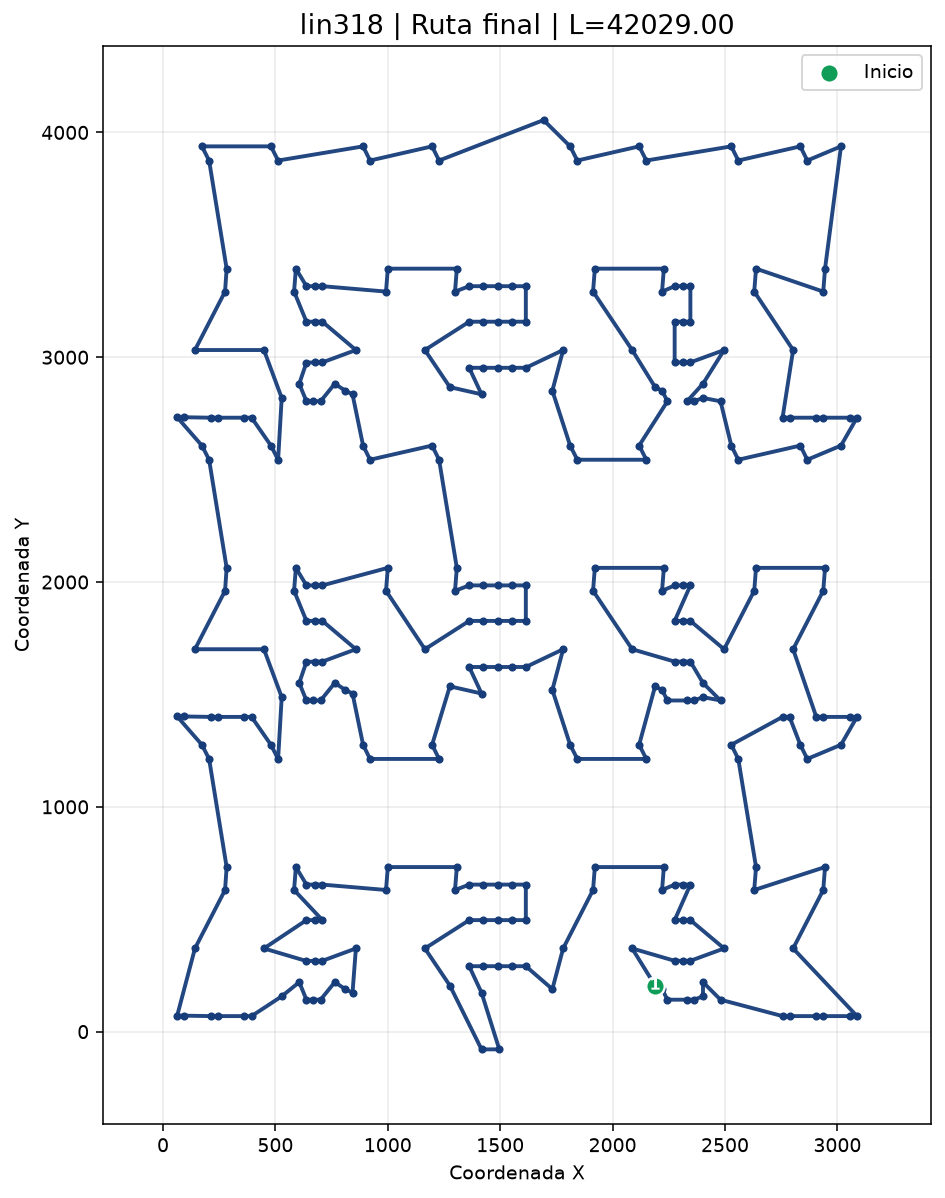
\includegraphics[width=0.80\textwidth]{Resultados_v2/LIN318.png}
\caption{Tour de largo 42\,029 (la BKS) encontrado en \texttt{lin318} en
0.45~s.}
\label{fig:lin318-route}
\end{figure}

\begin{figure}
\centering
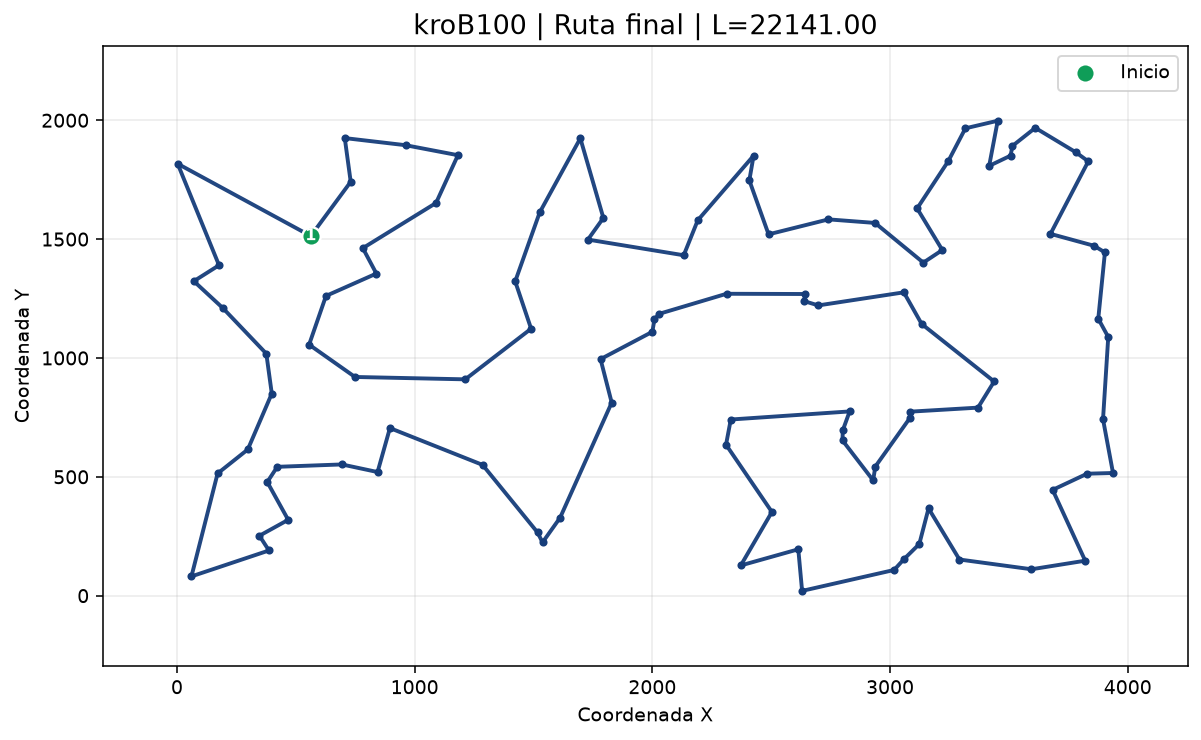
\includegraphics[width=0.80\textwidth]{Resultados_v2/KROB100.png}
\caption{Tour óptimo en \texttt{kroB100} (22\,141).}
\label{fig:krob100-route}
\end{figure}

\begin{figure}
\centering
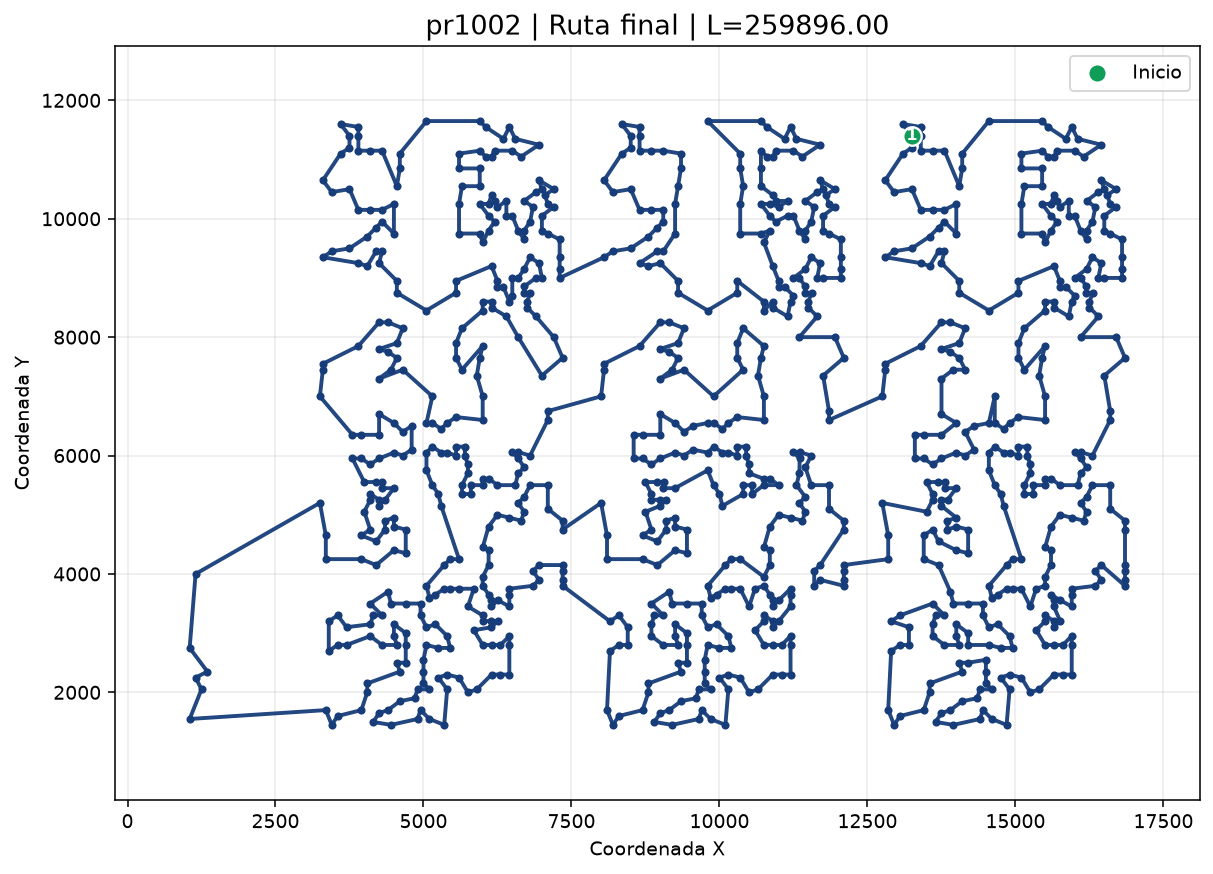
\includegraphics[width=0.80\textwidth]{Resultados_v2/PR1002.png}
\caption{Tour encontrado en \texttt{pr1002} en una sola ejecución
(259\,896, 0.329\% sobre la BKS).}
\label{fig:pr1002-route}
\end{figure}

\begin{figure}
\centering
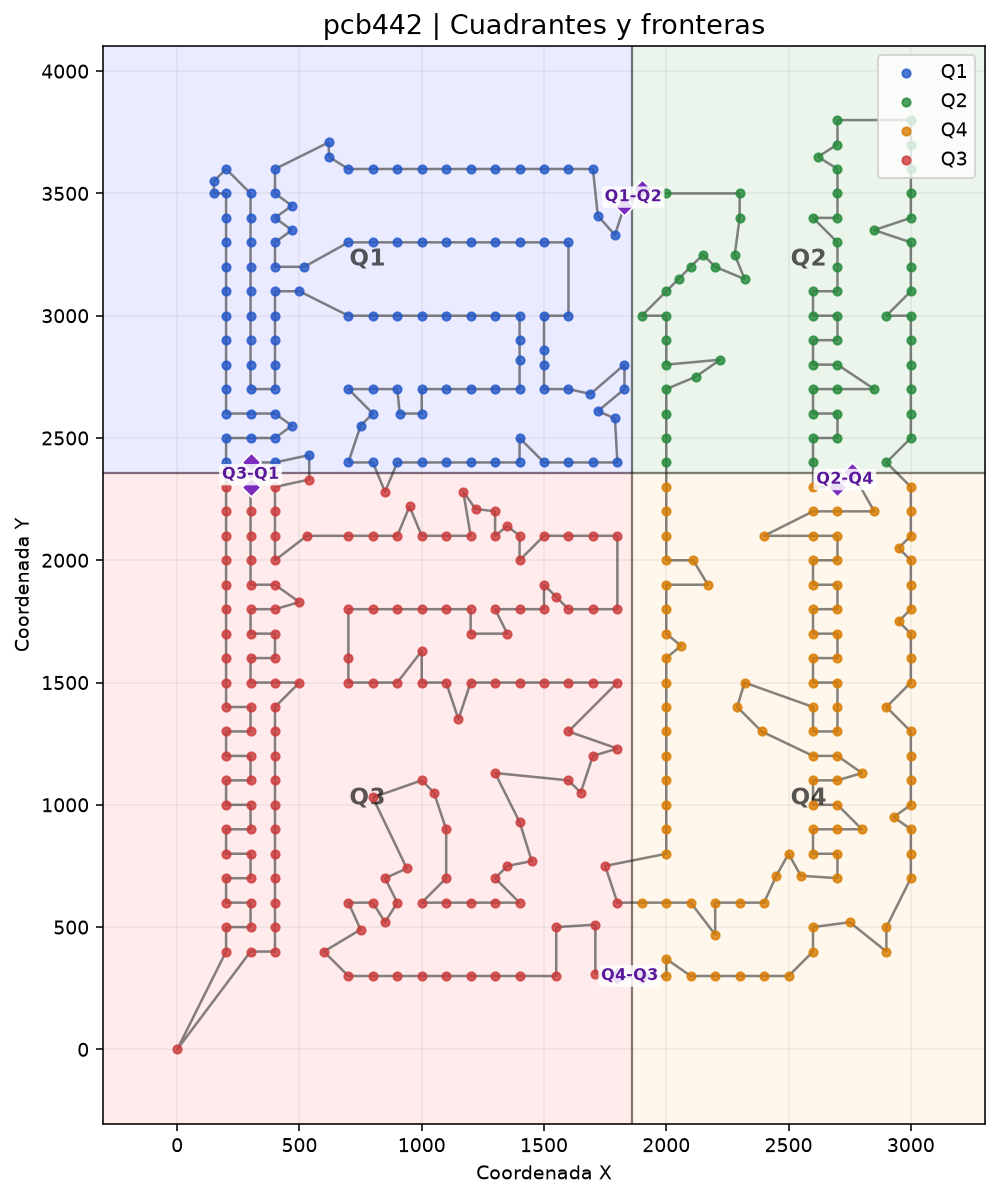
\includegraphics[width=0.80\textwidth]{Resultados_v2/PCB442_QUADRANTS.png}
\caption{Tour óptimo en \texttt{pcb442} (50\,778) coloreado por
cuadrante, con los cuatro pares de frontera elegidos.}
\label{fig:pcb442-quad}
\end{figure}

% ================================================================
\section{Discusión}
\label{sec:analysis}
% ================================================================

La ablación de la Sección~\ref{sec:ablation} precisa los roles de las dos
etapas. La construcción guiada por fronteras produce los mejores tours
iniciales: 9.95\% sobre la BKS frente a 24.71\% del vecino más cercano y
23.50\% de una partición sin pares de frontera. También entrega la mayor
cantidad de aciertos de la BKS y el menor GAP promedio tras el ILS. Sin
embargo, el motor de mejora explica la mayor parte de la calidad final.
Incluso los tours aleatorios terminan a menos de 0.12\% de la BKS en
promedio, y las diferencias entre construcciones después del ILS no son
estadísticamente significativas, salvo frente al inicio aleatorio. La
lectura honesta es, por lo tanto, que GSPH-FC es una construcción
geométrica que hace más confiable la búsqueda, acoplada a un ILS
localizado eficiente que hace la mayor parte del trabajo. Como las
perturbaciones son locales y cada movimiento es una inversión
registrada, una iteración cuesta microsegundos, y eso es lo que permite
alcanzar la BKS en todas las instancias de hasta 300 ciudades en mucho
menos de un segundo.

Frente a LKH (Sección~\ref{sec:lkh}), GSPH-FC solo es competitivo en
instancias pequeñas. Por encima de 300 ciudades LKH es más preciso
incluso con igual tiempo, lo que refleja los movimientos de profundidad
variable, mucho más fuertes, de la búsqueda tipo Lin--Kernighan.
Vemos a GSPH-FC como una alternativa transparente y liviana, con un
control claro entre tiempo y calidad, y no como un reemplazo de LKH.

Quedan cuatro limitaciones. Primero, por encima de unas 10\,000
ciudades la representación con arreglos hace que cada inversión de 2-opt
cueste $O(n)$, las ejecuciones llegan al tope de 60~s antes del
estancamiento y la matriz densa de distancias ($4n^2$ bytes) se
convierte en el cuello de botella de memoria. Segundo, las instancias muy
agrupadas, como \texttt{fl3795}, muestran una mayor dispersión entre
ejecuciones, lo que sugiere que las perturbaciones que cruzan entre
grupos están subrepresentadas. Tercero, la partición alineada con los
ejes puede no ser la mejor para instancias alargadas o agrupadas en
diagonal, y el método depende de la métrica: los valores históricos de
BKS con otra convención, como en \texttt{linhp318}, deben tratarse con
cuidado. Cuarto, los parámetros se ajustaron en seis instancias, y la
ablación y la comparación con LKH cubren instancias de hasta 2\,000
ciudades con 3--5 ejecuciones cada una; estudios más amplios precisarían
las pequeñas diferencias entre construcciones.

Como pasos siguientes prometedores están un movimiento de profundidad
variable (tipo Or-3opt o Lin--Kernighan) dentro del mismo esquema de
inversiones, listas doblemente enlazadas de dos niveles y distancias
calculadas al vuelo para las instancias más grandes, y orientaciones de
partición adaptativas.

% ================================================================
\section{Conclusiones}
\label{sec:conclusions}
% ================================================================

Presentamos \textbf{GSPH-FC}, una heurística para el TSP euclidiano cuya
característica central es hacer de la conectividad de fronteras un
principio de construcción de primer orden, junto con un motor de pulido
rediseñado: un ILS con parada por estancamiento, perturbaciones
double-bridge localizadas, aceptación de Metropolis y deshacer mediante
un registro de inversiones, ejecutado por núcleos compilados. En 77
instancias de TSPLIB el método alcanza la BKS en 44, incluidas todas las
de $n\le 300$, y se mantiene a menos de 0.60\% de la BKS hasta 6\,000
ciudades. Frente a la implementación anterior mejora a la vez la calidad
y la velocidad: las 37 instancias comparables alcanzan ahora la BKS,
unas 65 veces más rápido. Una ablación de la construcción muestra que la
conectividad de fronteras entrega los mejores tours iniciales y los
resultados más consistentes, mientras que el ILS localizado explica la
mayor parte de la calidad final. Un estudio de sensibilidad respalda los
parámetros elegidos, y una comparación con LKH-3 sitúa a GSPH-FC como una
alternativa liviana e interpretable que iguala a LKH en instancias
pequeñas, pero no por encima de 300 ciudades. El trabajo futuro se
centrará en movimientos de profundidad variable dentro del mismo esquema
de inversiones, en estructuras de datos que extiendan el método a
instancias de decenas de miles de ciudades y en costos asimétricos
provenientes de redes viales reales.

% REVISIÓN CIEGA: agradecimientos ocultos
%
% RESTAURAR ANTES DE LA VERSIÓN FINAL:
%\begin{credits}
%\subsubsection{\ackname}
%Los autores agradecen al equipo docente del curso de Heurísticas de la
%Universidad Andrés Bello por su orientación y apoyo material durante el
%desarrollo de este trabajo.
%\end{credits}

\bibliographystyle{splncs04}
\bibliography{bibliografia}

\end{document}
